\documentclass[12pt, border=12pt]{standalone}
\usepackage[utf8]{inputenc}
\usepackage[utf8]{vietnam}
\usepackage{amsmath,amsfonts,amssymb}
\usepackage{type1cm}
\usepackage{graphicx}
\usepackage{multirow}
\usepackage{multicol}
\usepackage{array}
\usepackage{comment}
\usepackage[unicode]{hyperref}
\usepackage{tikz}
\usepackage{color}
\usepackage[american,cuteinductors,smartlabels]{circuitikz}
\usetikzlibrary{arrows}
\usepackage{tikz}
\usetikzlibrary{calc,patterns,angles,quotes}
\usetikzlibrary{arrows, decorations.markings, calc, fadings, decorations.pathreplacing, patterns, decorations.pathmorphing, positioning}	
%\tikzstyle{every path}=[line width=1.2pt]

\tikzset{middlearrow/.style={
        decoration={markings,
            mark= at position 0.5 with {\arrow{#1}} ,
        },
        postaction={decorate}
    }
}
\begin{document}
	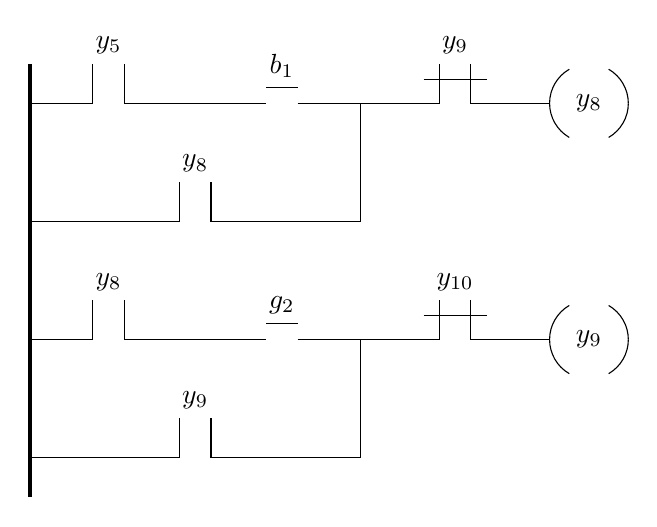
\begin{tikzpicture}[>=triangle 45]
		\draw[ultra thick] (8.5,0.5) -- (8.5,-5);
						
		\draw (8.5,0) -- (9.3,0) -- (9.3,0.5); \draw (9.7,0.5) -- (9.7,0) -- (11.5,0); \draw (9.5,0.5) node[above]{$y_5$}; \draw (11.5,0.2) -- (11.9,0.2); \draw(11.7,0.2) node[above]{$b_1$}; \draw (11.9,0) -- (12.7,0); \draw (12.7,0) -- (13.7,0)-- (13.7,0.5); \draw (14.1,0.5) -- (14.1,0)-- (15.1,0); \draw (13.5,0.3) -- (14.3, 0.3); \draw (13.9,0.5) node[above]{$y_9$};  \draw (15.1,0) arc (180:120:.5);\draw (15.1,0) arc (180:240:.5); \draw (16.1,0) arc (0:60:.5);\draw (16.1,0) arc (0:-60:.5); \draw (15.6,0) node{$y_8$}; \draw (8.5,-1.5) -- (10.4,-1.5) -- (10.4,-1); \draw (10.8,-1) -- (10.8,-1.5)-- (12.7,-1.5) -- (12.7,0); \draw (10.6,-1) node[above]{$y_8$};
						
	\draw (8.5,-3) -- (9.3,-3) -- (9.3,-2.5); \draw (9.7,-2.5) -- (9.7,-3) -- (11.5,-3); \draw (9.5,-2.5) node[above]{$y_8$};  \draw (11.5,-2.8) -- (11.9,-2.8); \draw(11.7,-2.8) node[above]{$g_2$}; \draw (11.9,-3) -- (12.7,-3); \draw (12.7,-3) -- (13.7,-3)-- (13.7,-2.5); \draw (14.1,-2.5) -- (14.1,-3) -- (15.1,-3); \draw (13.5,-2.7) -- (14.3, -2.7); \draw (13.9,-2.5) node[above]{$y_{10}$};\draw (15.1,-3) arc (180:120:.5);\draw (15.1,-3) arc (180:240:.5); \draw (16.1,-3) arc (0:60:.5);\draw (16.1,-3) arc (0:-60:.5); \draw (15.6,-3) node{$y_9$}; \draw (8.5,-4.5) -- (10.4,-4.5) -- (10.4,-4); \draw (10.8,-4) -- (10.8,-4.5)-- (12.7,-4.5) -- (12.7,-3); \draw (10.6,-4) node[above]{$y_9$};
	\end{tikzpicture}
\end{document}